\section{Εισαγωγή}
Ο κώδικας όλων των παραδειγμάτων βρίσκεται στο \href{https://github.com/chgogos/ceteiep_dsa}{https://github.com/chgogos/ceteiep\_dsa}.

\section{Σωροί}
Ο σωρός είναι μια μερικά ταξινομημένη δομή δεδομένων. Υπάρχουν δύο ειδών σωροί, ο σωρός μεγίστων (Max-Heap) και ο σωρός ελαχίστων (Min-Heap). Οι ιδιότητες των σωρών που θα περιγραφούν στη συνέχεια αφορούν τους σωρούς μεγίστων αλλά αντίστοιχες ιδιότητες ισχύουν και για τους σωρούς ελαχίστων. Ειδικότερα, ένας σωρός μεγίστων υποστηρίζει ταχύτατα τις ακόλουθες λειτουργίες:
\begin{itemize}[noitemsep]
\item Εύρεση του στοιχείου με τη μεγαλύτερη τιμή κλειδιού.
\item Διαγραφή του στοιχείου με τη μεγαλύτερη τιμή κλειδιού.
\item Εισαγωγή νέου κλειδιού στη δομή.
\end{itemize}

Ένας σωρός μπορεί να θεωρηθεί ως ένα δυαδικό δένδρο για το οποίο ισχύουν οι ακόλουθοι δύο περιορισμοί:
\begin{itemize}[noitemsep]
\item	Πληρότητα: το δυαδικό δένδρο είναι συμπληρωμένο, δηλαδή όλα τα επίπεδά του είναι πλήρως συμπληρωμένα εκτός πιθανά από το τελευταίο επίπεδο στο οποίο μπορούν να λείπουν μόνο κάποια από τα δεξιότερα φύλλα.
\item	Κυριαρχία γονέα: το κλειδί σε κάθε κορυφή είναι μεγαλύτερο ή ίσο από τα κλειδιά των παιδιών (σε Max-Heap).
\end{itemize}

Στο σχήμα \ref{fig:heap1} παρουσιάζεται ένα παράδειγμα σωρού μεγίστων στη δενδρική του μορφή.

\begin{figure}[ht]
\centering
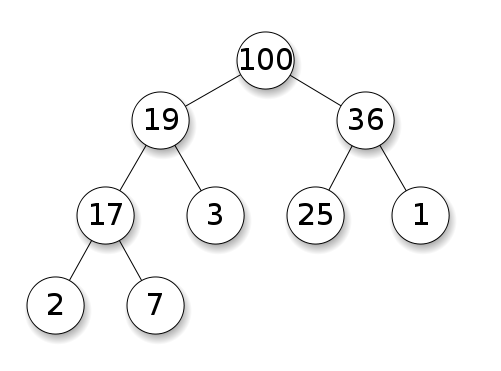
\includegraphics[width=100mm]{heap1.png}
\caption{Σωρός μεγίστων στη δενδρική του απεικόνιση}
\label{fig:heap1}
\end{figure}

Ένας σωρός μπορεί να υλοποιηθεί με ένα πίνακα καταγράφοντας στον πίνακα στη σειρά τα στοιχεία του δυαδικού δένδρου από αριστερά προς τα δεξιά και από πάνω προς τα κάτω (σχήμα \ref{fig:heap2}). Μερικές σημαντικές ιδιότητες οι οποίες προκύπτουν εφόσον τηρηθεί ο παραπάνω τρόπος αντιστοίχισης των στοιχείων του δένδρου στα στοιχεία του  πίνακα είναι οι ακόλουθες:
\begin{itemize}[noitemsep]
\item	Στον πίνακα τα κελιά γονείς βρίσκονται στις πρώτες $\lfloor{\frac{n}{2}}\rfloor$ θέσεις ενώ τα φύλλα καταλαμβάνουν τις υπόλοιπες θέσεις. 
\item	Στον πίνακα τα παιδιά για κάθε κλειδί στις θέσεις $i$ από 1 μέχρι και $\lfloor{\frac{n}{2}}\rfloor$ βρίσκονται στις θέσεις $2*i$ και $2*i + 1$.
\item	Στον πίνακα ο γονέας για κάθε κλειδί στις θέσεις $i$ από 2 μέχρι και $n$ βρίσκεται στη θέση $\lfloor{\frac{i}{2}}\rfloor$.
\end{itemize}

\begin{figure}[ht]
\centering
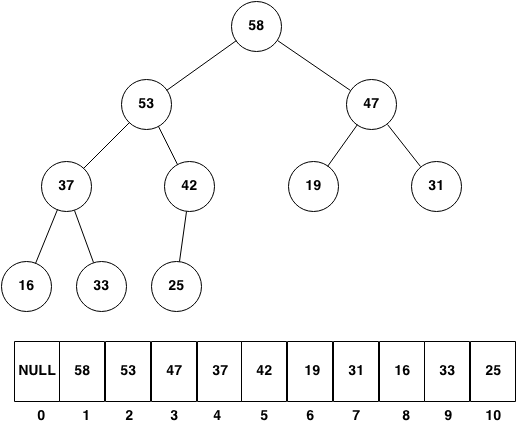
\includegraphics[width=100mm]{heap2.png}
\caption{Αναπαράσταση ενός σωρού μεγίστων ως πίνακα}
\label{fig:heap2}
\end{figure}

\section{Υλοποίηση ενός σωρού}
Στη συνέχεια παρουσιάζεται η υλοποίηση ενός σωρού μεγίστων που περιέχει ακέραιες τιμές-κλειδιά.

\lstinputlisting[caption = Σωρός μεγίστων ακεραίων (max\_heap.cpp)]{lab06/max_heap.cpp}

Ο ακόλουθος κώδικας χρησιμοποιεί τη συνάρτηση heap\_bottom\_up και μέσω αυτής τη συνάρτηση heapify προκειμένου να μετασχηματίσει έναν πίνακα ακεραίων σε σωρό μεγίστων.
\lstinputlisting[caption = Δημιουργία σωρού από πίνακα με heapify (heap1.cpp)]{lab06/heap1.cpp}

\lstinputlisting[style=DOS]{lab06/heap1.out}

Ο ακόλουθος κώδικας δημιουργεί σταδιακά έναν σωρό εισάγοντας δέκα τιμές με τη συνάρτηση insert\_key. Στη συνέχεια πραγματοποιούνται εξαγωγές τιμών με τη συνάρτηση maximum\_key\_deletion μέχρι ο σωρός να αδειάσει.

\lstinputlisting[caption = Δημιουργία σωρού με εισαγωγές τιμών και εν συνεχεία άδειασμα του σωρού με διαδοχικές διαγραφές της μέγιστης τιμής (heap2.cpp)]{lab06/heap2.cpp}

\lstinputlisting[style=DOS]{lab06/heap2.out}


\section{Ταξινόμηση Heapsort}
Ο αλγόριθμος Heapsort προτάθηκε από τον J.W.J.Williams το 1964 και αποτελείται από 2 στάδια:
\begin{itemize}[noitemsep]
\item Δημιουργία σωρού με τα n στοιχεία ενός πίνακα τα στοιχεία του οποίου ζητείται να ταξινομηθούν. 
\item Εφαρμογή της διαγραφής της ρίζας n -1 φορές.
\end{itemize}
Το αποτέλεσμα είναι ότι τα στοιχεία αφαιρούνται από το σωρό σε φθίνουσα σειρά. Καθώς κατά την αφαίρεσή του κάθε στοιχείου, αυτό τοποθετείται στο τέλος του σωρού, τελικά ο σωρός περιέχει τα αρχικά δεδομένα σε αύξουσα σειρά. Στη συνέχεια παρουσιάζεται η υλοποίηση του αλγορίθμου HeapSort. Επιπλέον ο κώδικας ταξινομεί πίνακες μεγέθους 10.000, 20.000, 40.000 80.000 και 100.000 που περιέχουν τυχαίες ακέραιες τιμές και πραγματοποιείται σύγκριση με τους χρόνους εκτέλεσης που επιτυγχάνει η std::sort.

\lstinputlisting[caption = Ο αλγόριθμος heapsort (heapsort.cpp)]{lab06/heapsort.cpp}

\lstinputlisting[style=DOS]{lab06/heapsort.out}


\section{Η δομή priority\_queue της STL}
Η STL της C++ περιέχει υλοποίηση της δομής std::priority\_queue (ουρά προτεραιότητας) η οποία είναι ένας σωρός μεγίστων. Κάθε στοιχείο που εισέρχεται  στην ουρά προτεραιότητας έχει μια προτεραιότητα που συνδέεται με αυτό και το στοιχείο με τη μεγαλύτερη προτεραιότητα βρίσκεται πάντα στην αρχή της ουράς. Οι κυριότερες λειτουργίες που υποστηρίζονται από την std::priority\_queue είναι οι ακόλουθες:
\begin{itemize}[noitemsep]
\item push: εισαγωγή ενός στοιχείου στη δομή
\item top: επιστροφή χωρίς εξαγωγή του στοιχείου με τη μεγαλύτερη προτεραιότητα
\item pop: απώθηση του στοιχείου με τη μεγαλύτερη προτεραιότητα
\item size: πλήθος των στοιχείων που υπάρχουν στη δομή
\item empty: επιστρέφει true αν η δομή είναι άδεια αλλιώς επιστρέφει false
\end{itemize}
Ένα παράδειγμα χρήσης της std::priority\_queue ως σωρού μεγίστων αλλά και ως σωρού ελαχίστων παρουσιάζεται στη συνέχεια.

\lstinputlisting[caption = Παράδειγμα με priority\_queue της STL (stl\_priority\_queue.cpp)]{lab06/stl_priority_queue.cpp}

\lstinputlisting[style=DOS]{lab06/stl_priority_queue.out}


\section{Παραδείγματα}
\subsection{Παράδειγμα 1}
Διάμεσος ενός δείγματος Ν παρατηρήσεων οι οποίες έχουν διαταχθεί σε αύξουσα σειρά ορίζεται ως η μεσαία παρατήρηση, όταν το Ν είναι περιττός αριθμός, ή ο μέσος όρος (ημιάθροισμα) των δύο μεσαίων παρατηρήσεων όταν το Ν είναι άρτιος αριθμός. 
Έστω ότι για διάφορες τιμές που παράγονται με κάποιον τρόπο ζητείται ο υπολογισμός της διάμεσης  τιμής καθώς παράγεται κάθε νέα τιμή και για όλες τις τιμές που έχουν προηγηθεί μαζί με την τρέχουσα τιμή όπως φαίνεται στο επόμενο παράδειγμα:\\ 
5  $\Rightarrow$  διάμεσος 5\\
5, 7 $\Rightarrow$ διάμεσος 6\\
5, 7, 13 $\Rightarrow$ διάμεσος 7\\
5, 7, 13, 12 $\Rightarrow$ 5, 7, 12, 13 $\Rightarrow$ διάμεσος 9.5\\
5, 7, 13, 12, 2 $\Rightarrow$ 2, 5, 7, 12, 13 $\Rightarrow$ διάμεσος 7

\lstinputlisting[caption = Υπολογισμός διαμέσου σε μια ροή τιμών (lab06\_ex1.cpp)]{lab06/lab06_ex1.cpp}

\lstinputlisting[style=DOS]{lab06/lab06_ex1.out}


\subsection{Παράδειγμα 2}

\section{Ασκήσεις}
\begin{enumerate}
\item a
\item b
\item Να υλοποιηθεί ο σωρός μεγίστων που παρουσιάστηκε στον κώδικα Χ ως κλάση. 
\item d
\end{enumerate}

\begin{thebibliography}{9}
\bibitem{cppexceptions}
Geeks for Geeks, Priority Queue in C++ Standard Template Library (STL), \href{http://www.geeksforgeeks.org/priority-queue-in-cpp-stl/}{http://www.geeksforgeeks.org/priority-queue-in-cpp-stl/}
\end{thebibliography}

